\documentclass[border=2pt]{standalone}
\usepackage{pgfplots}
\usepackage{xcolor}

\pgfplotsset{compat=1.18}

\definecolor{Garnet}{HTML}{73000A}
\definecolor{Gray10}{gray}{0.10}
\definecolor{Gray30}{gray}{0.30}
\definecolor{Gray50}{gray}{0.50}
\definecolor{Gray70}{gray}{0.70}
\definecolor{Gray90}{gray}{0.90}

\pgfplotsset{
  every axis/.style={
    axis line style={draw=black, line width=0.6pt},
    tick style={draw=black, line width=0.6pt},
    tick label style={font=\footnotesize\color{black}},
    label style={font=\small\color{black}},
    grid=both,
    grid style={draw=Gray90, line width=0.3pt},
    legend style={
      draw=none,
      font=\footnotesize\color{black},
      fill=white,
      at={(0.95,0.05)},
      anchor=south east,
    },
  },
  linestyle/.style={
    line width=0.8pt,
    mark=none,
  },
}

\begin{document}

% YOLOv12-L Single mAP50
\begin{figure}[h]
\centering
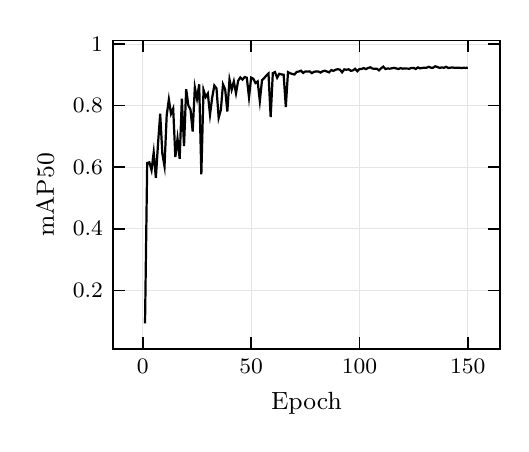
\begin{tikzpicture}
\begin{axis}[
  xlabel={Epoch},
  ylabel={mAP50},
  width=6.5cm,
  height=5.5cm,
]
\addplot[linestyle, color=black] coordinates {
  (1,0.092880)
  (2,0.613970)
  (3,0.615930)
  (4,0.590480)
  (5,0.647800)
  (6,0.565330)
  (7,0.676310)
  (8,0.773430)
  (9,0.643890)
  (10,0.603230)
  (11,0.768220)
  (12,0.820120)
  (13,0.773670)
  (14,0.790700)
  (15,0.633410)
  (16,0.693250)
  (17,0.627530)
  (18,0.822720)
  (19,0.668560)
  (20,0.853410)
  (21,0.800540)
  (22,0.786930)
  (23,0.715710)
  (24,0.859330)
  (25,0.822680)
  (26,0.869140)
  (27,0.576660)
  (28,0.850880)
  (29,0.828110)
  (30,0.839380)
  (31,0.770500)
  (32,0.825840)
  (33,0.865260)
  (34,0.855920)
  (35,0.760320)
  (36,0.785880)
  (37,0.868920)
  (38,0.852780)
  (39,0.781090)
  (40,0.884590)
  (41,0.851680)
  (42,0.878480)
  (43,0.840180)
  (44,0.880700)
  (45,0.891500)
  (46,0.884480)
  (47,0.892800)
  (48,0.890630)
  (49,0.826860)
  (50,0.891010)
  (51,0.887410)
  (52,0.873340)
  (53,0.878560)
  (54,0.814970)
  (55,0.882150)
  (56,0.889210)
  (57,0.897640)
  (58,0.904250)
  (59,0.762760)
  (60,0.905420)
  (61,0.909020)
  (62,0.890640)
  (63,0.903380)
  (64,0.901200)
  (65,0.900590)
  (66,0.795560)
  (67,0.908740)
  (68,0.905020)
  (69,0.902790)
  (70,0.901060)
  (71,0.909240)
  (72,0.910640)
  (73,0.913540)
  (74,0.905980)
  (75,0.910890)
  (76,0.910390)
  (77,0.911230)
  (78,0.905490)
  (79,0.909830)
  (80,0.910980)
  (81,0.911010)
  (82,0.907300)
  (83,0.911440)
  (84,0.913450)
  (85,0.910630)
  (86,0.908190)
  (87,0.915350)
  (88,0.912780)
  (89,0.916570)
  (90,0.918400)
  (91,0.916660)
  (92,0.908220)
  (93,0.917750)
  (94,0.916430)
  (95,0.918120)
  (96,0.913030)
  (97,0.914560)
  (98,0.919740)
  (99,0.911850)
  (100,0.918600)
  (101,0.919260)
  (102,0.921750)
  (103,0.918700)
  (104,0.922120)
  (105,0.924400)
  (106,0.920370)
  (107,0.919520)
  (108,0.919990)
  (109,0.914460)
  (110,0.921250)
  (111,0.926610)
  (112,0.918810)
  (113,0.920550)
  (114,0.919870)
  (115,0.921360)
  (116,0.922660)
  (117,0.920770)
  (118,0.919000)
  (119,0.921700)
  (120,0.919920)
  (121,0.920980)
  (122,0.920230)
  (123,0.919910)
  (124,0.922360)
  (125,0.922450)
  (126,0.919150)
  (127,0.924180)
  (128,0.921000)
  (129,0.922430)
  (130,0.923160)
  (131,0.923120)
  (132,0.925950)
  (133,0.923240)
  (134,0.923260)
  (135,0.927680)
  (136,0.925240)
  (137,0.922560)
  (138,0.924080)
  (139,0.922980)
  (140,0.926070)
  (141,0.922230)
  (142,0.923170)
  (143,0.923890)
  (144,0.922500)
  (145,0.923030)
  (146,0.923340)
  (147,0.921960)
  (148,0.922910)
  (149,0.922470)
  (150,0.923090)
};
\end{axis}
\end{tikzpicture}
\end{figure}

% YOLOv12-L Single mAP50-95
\begin{figure}[h]
\centering
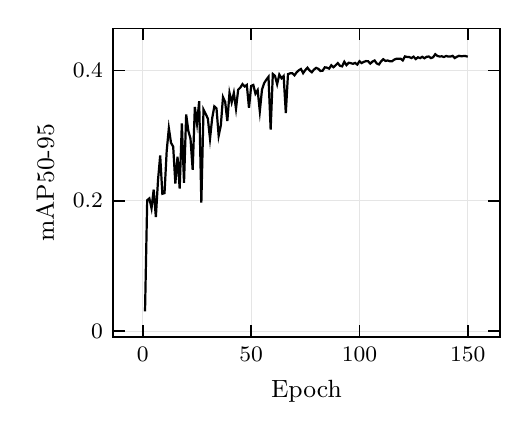
\begin{tikzpicture}
\begin{axis}[
  xlabel={Epoch},
  ylabel={mAP50-95},
  width=6.5cm,
  height=5.5cm,
]
\addplot[linestyle, color=black] coordinates {
  (1,0.030330)
  (2,0.200930)
  (3,0.203700)
  (4,0.188610)
  (5,0.217180)
  (6,0.174930)
  (7,0.231970)
  (8,0.269470)
  (9,0.210760)
  (10,0.211860)
  (11,0.276310)
  (12,0.311380)
  (13,0.289000)
  (14,0.283110)
  (15,0.226600)
  (16,0.267790)
  (17,0.218660)
  (18,0.318910)
  (19,0.227640)
  (20,0.332490)
  (21,0.307340)
  (22,0.295310)
  (23,0.247620)
  (24,0.344170)
  (25,0.318600)
  (26,0.352810)
  (27,0.197100)
  (28,0.339910)
  (29,0.333350)
  (30,0.326290)
  (31,0.295240)
  (32,0.326670)
  (33,0.344940)
  (34,0.341870)
  (35,0.299810)
  (36,0.315920)
  (37,0.359170)
  (38,0.351670)
  (39,0.322440)
  (40,0.365690)
  (41,0.351070)
  (42,0.365590)
  (43,0.341330)
  (44,0.370530)
  (45,0.373780)
  (46,0.379150)
  (47,0.375520)
  (48,0.377840)
  (49,0.342630)
  (50,0.376260)
  (51,0.377850)
  (52,0.364370)
  (53,0.369810)
  (54,0.337390)
  (55,0.370720)
  (56,0.380590)
  (57,0.385910)
  (58,0.390360)
  (59,0.309390)
  (60,0.394630)
  (61,0.391790)
  (62,0.379020)
  (63,0.393790)
  (64,0.388200)
  (65,0.391650)
  (66,0.334760)
  (67,0.394470)
  (68,0.395650)
  (69,0.395840)
  (70,0.392560)
  (71,0.397280)
  (72,0.400350)
  (73,0.402320)
  (74,0.395960)
  (75,0.400650)
  (76,0.404360)
  (77,0.400020)
  (78,0.397320)
  (79,0.401480)
  (80,0.404060)
  (81,0.402600)
  (82,0.399290)
  (83,0.399720)
  (84,0.404920)
  (85,0.404400)
  (86,0.402880)
  (87,0.408100)
  (88,0.405070)
  (89,0.408020)
  (90,0.411320)
  (91,0.407180)
  (92,0.406410)
  (93,0.413450)
  (94,0.408290)
  (95,0.411930)
  (96,0.411300)
  (97,0.410300)
  (98,0.411680)
  (99,0.409070)
  (100,0.414290)
  (101,0.411380)
  (102,0.413220)
  (103,0.414470)
  (104,0.414300)
  (105,0.410590)
  (106,0.413700)
  (107,0.415390)
  (108,0.410750)
  (109,0.409300)
  (110,0.414080)
  (111,0.417320)
  (112,0.414770)
  (113,0.415390)
  (114,0.414300)
  (115,0.414120)
  (116,0.416630)
  (117,0.417950)
  (118,0.417950)
  (119,0.418160)
  (120,0.415460)
  (121,0.421670)
  (122,0.420760)
  (123,0.420660)
  (124,0.419150)
  (125,0.421250)
  (126,0.417620)
  (127,0.420270)
  (128,0.419050)
  (129,0.421060)
  (130,0.418820)
  (131,0.421060)
  (132,0.421510)
  (133,0.419060)
  (134,0.420350)
  (135,0.425020)
  (136,0.422310)
  (137,0.421560)
  (138,0.421820)
  (139,0.420680)
  (140,0.422370)
  (141,0.421370)
  (142,0.421410)
  (143,0.422510)
  (144,0.419150)
  (145,0.421170)
  (146,0.422590)
  (147,0.421900)
  (148,0.422180)
  (149,0.422170)
  (150,0.421220)
};
\end{axis}
\end{tikzpicture}
\end{figure}



\end{document}
